\section{Model analityczny}
Celem niniejszego rozdziału jest zdefiniowanie, jak wyglądać będzie architektura tworzonego systemu. Aby to osiągnąć, w~rozdziale załączone zostały diagramy wykonane zgodnie ze~standardem UML, które stanowią wizualną reprezentację architektury systemu oraz pozwalają na~łatwiejszą analizę stanu projektu.

\subsection{Diagram klas}
Przedstawiony poniżej diagram klas reprezentuje wszystkie wykorzystywane przez Zleceniodawcę elementy składające się na cały system. Diagram ten jest kluczowy przede wszystkim dla deweloperów oraz innych osób zajmujących się bezpośrednio wytwarzaniem oprogramowania, tym niemniej powinien zostać zatwierdzony także przez przedstawicieli Zleceniodawcy -- diagram klas jest bowiem punktem łączącym -- z~jednej strony wyobrażenie klienta o~podziale funkcjonalności, a~z~drugiej decyzje projektowe podjęte przez zespół zajmujący się implementacją.\\

\begin{figure}[H]
  \centering
  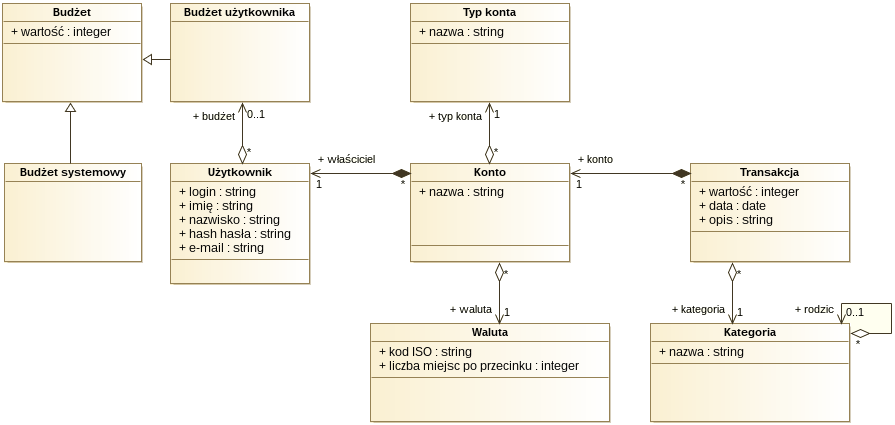
\includegraphics[width=\textwidth]{images/class-diagram.png}
  \caption{Diagram klas systemu.}
\end{figure}

Diagram klas obrazuje zależności (agregacje, kompozycje, relacje dziedziczenia) pomiędzy poszczególnymi klasami na~tyle szczegółowo, by~osoby nieposiadające wykształcenia informatycznego i~nieznające metod programowania obiektowego mogły zrozumieć zasadę podziału bez szczegółowych wyjaśnień. Wszystkie atrybuty czy operacje ważne z~punktu widzenia Zleceniodawcy, które mogą mieć wpływ na~ocenę projektu zostały umieszczone na~diagramie. Poniżej umieszczony został opis każdej z~klas.\\

\textbf{Użytkownik} reprezentuję osobę korzystającą z~aplikacji. Klasa ta~zawiera istotne informacje potrzebne głównie do~uwierzytelniania, takie jak login oraz hash hasła. Pozostałe pola to~na~przykład imię i~nazwisko, czy adres e-mail.\\

\textbf{Konto} jest klasą reprezentującą konto pieniężne (np. oszczędnościowe, osobiste, czy walutowe), które należy do~danego użytkownika. Klasa ta~posiada pola, takie jak nazwa, typ, waluta oraz bieżące saldo.\\

\textbf{Typ konta} jest klasą wydzieloną z~klasy Konto. Utworzenie tej klasy pozwoli na~ograniczenie wartości wprowadzanych w~polu typ konta.\\

\textbf{Waluta} jest kolejną klasą wydzieloną z~klasy Konto. Utworzenie tej klasy pozwoli na~ograniczenie wartości wprowadzanych w~polu waluta. Ponadto przechowuje ona liczbę miejsc po~przecinku, na~jakie zezwala dana waluta, a~więc pozwoli na~walidację wartości pieniężnych wprowadzanych przez użytkownika do~systemu.\\

\textbf{Transakcja} reprezentuje przepływ pieniędzy między kontami. Istnieją trzy typy transakcji -- przychody (pieniądze pochodzące z~konta poza systemem, które trafiają na~jedno z~kont użytkownika), koszty (pieniądze pochodzące z~jednego z~kont użytkownika, które trafiają na~konto poza systemem), lub przelew (pieniądze transferowane pomiędzy dwoma kontami, oba należące do tego samego użytkownika). Klasa ta~zawiera także inne pola, takie jak data, opis (opcjonalnie), czy wartość pieniężna.\\

\textbf{Kategoria} reprezentuje etykiety, które mogą być przypisane do~transakcji. Podobnie jak klasy Waluta oraz Typ konta, jest to~klasa wydzielona z~innej klasy, w~tym przypadku z~Transakcji. Zawiera tylko pole przechowujące nazwę. Kategorie tworzą strukturę drzewa -- jest to~dozwolone poprzez rekurencyjną relację jeden-do-wielu.\\

\textbf{Budżet} jest klasą abstrakcyjną reprezentującą budżet, czyli ograniczenie nakładane na~użytkownika lub cały system. Zawiera ona~tylko jedno pole -- wartość ograniczenia. Istnieją dwie klasy dziedziczące po~klasie Budżet: Budżet użytkownika oraz Budżet systemowy, odpowiednio reprezentują one ograniczenia nałożone na~konkretnego użytkownika, lub cały system.\\

\subsection{Model bazy danych}
Ważnym elementem tworzonego systemu informatycznego jest baza danych przechowująca wszystkie informacje, które powinny być w~niej trwale. Jak opisano w~części dotyczącej sprzętu, wszystkie informacje powinny być przechowywane redundantnie, na~przynajmniej dwóch niezależnych od~siebie macierzach dyskowych. Pozwoli to na~uniknięcie problemów związanych z~ewentualnym awariami i~chwilowymi przerwami w~dostępności.

W~czasie tworzenia projektu bazy danych opierano się przede wszystkim na~stworzonym wcześniej diagramie klas. Większość klas została zamieniona na~odpowiadające im~tabele w~bazie danych. W~przypadku relacji wiele-do-wielu konieczne było stworzenie dodatkowych tabel łączących. Enumeracje zostały zamienione na~osobne tabele tylko w~uzasadnionych przypadkach.

Poniżej zaprezentowano model bazy danych wykorzystywanej w~tworzonym systemie.

\begin{figure}[H]
  \centering
  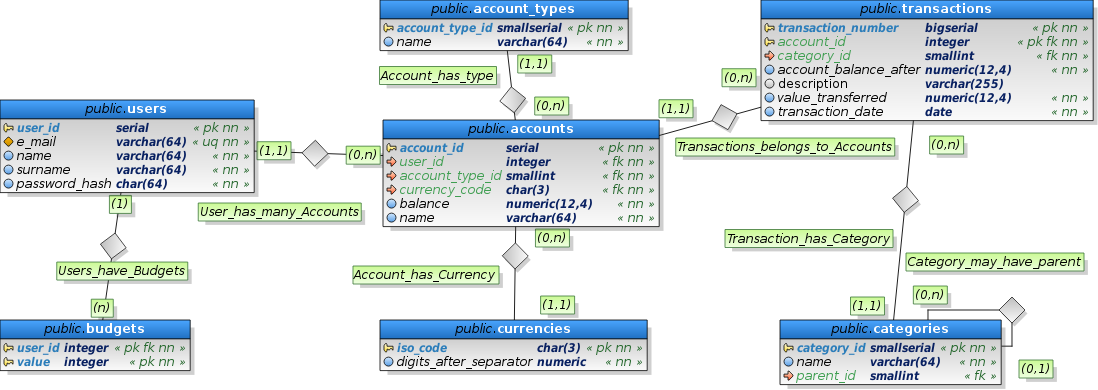
\includegraphics[width=1.4\textwidth,angle=90]{images/db.png}
  \caption{Model bazy danych systemu.}
\end{figure}

Poniżej znajdują się opisy każdej z~tabel w~bazie danych wraz z~wyjaśnieniem poszczególnych kolumn w~każdej z~nich.

\paragraph{Users} tabela przechowująca dane o~użytkownikach systemu.\\

\begin{tabular}{| c | p{4cm} | c | c |}
  \hline \textbf{Nazwa atrybutu} & \textbf{Opis} & \textbf{Typ danych} & \textbf{Ograniczenia} \\ \hline
  user\_id & PRIMARY KEY & serial & NOT NULL, UNIQUE \\ \hline
  e\_mail & adres elektroniczny użytkownika & varchar(64) & NOT NULL, UNIQUE \\ \hline
  name & imię użytkownika & varchar(64) & NOT NULL \\ \hline
  surname & nazwisko użytkownika & varchar(64) & NOT NULL \\ \hline
  password\_hash & hash hasła użytkownika & char(64) & NOT NULL \\ \hline
\end{tabular}

\paragraph{Accounts} tabela przechowująca dane o~kontach znajdujących się w~systemie.\\

\begin{tabular}{| c | p{4cm} | c | c |}
  \hline \textbf{Nazwa atrybutu} & \textbf{Opis} & \textbf{Typ danych} & \textbf{Ograniczenia} \\ \hline
  account\_id & PRIMARY KEY & serial & NOT NULL, UNIQUE \\ \hline
  user\_id & FOREIGN KEY & integer & NOT NULL \\ \hline
  account\_type\_id & FOREIGN KEY & smallint & NOT NULL \\ \hline
  currency\_code & FOREIGN KEY & char(3) & NOT NULL \\ \hline
  balance & aktualny stan konta & numeric(12,4) & NOT NULL \\ \hline
  name & nazwa konta & varchar(64) & NOT NULL \\ \hline
\end{tabular}

\paragraph{Account types} tabela przechowująca możliwe typy kont dostępne w~systemie.\\

\begin{tabular}{| c | p{4cm} | c | c |}
  \hline \textbf{Nazwa atrybutu} & \textbf{Opis} & \textbf{Typ danych} & \textbf{Ograniczenia} \\ \hline
  account\_type\_id & PRIMARY KEY & smallint & NOT NULL, UNIQUE \\ \hline
  name & nazwa typu konta & varchar(64) & NOT NULL \\ \hline
\end{tabular}

\paragraph{Currencies} tabela przechowująca dane o~walutach dostępnych w~systemie.\\

\begin{tabular}{| c | p{4cm} | c | c |}
  \hline \textbf{Nazwa atrybutu} & \textbf{Opis} & \textbf{Typ danych} & \textbf{Ograniczenia} \\ \hline
  iso\_code & PRIMARY KEY & char(3) & NOT NULL, UNIQUE \\ \hline
  digits\_after\_separator & liczba miejsc po przecinku w~danej walucie & numeric & NOT NULL \\ \hline
\end{tabular}

\newpage
\paragraph{Transactions} tabela przechowująca dane o~transakcjach.\\

\begin{tabular}{| c | p{4cm} | c | c |}
  \hline \textbf{Nazwa atrybutu} & \textbf{Opis} & \textbf{Typ danych} & \textbf{Ograniczenia} \\ \hline
  transaction\_number & PRIMARY KEY & bigserial & NOT NULL \\ \hline
  account\_id & FOREIGN KEY, PRIMARY KEY & serial & NOT NULL \\ \hline
  category\_id & FOREIGN KEY & smallint & NOT NULL \\ \hline
  value\_transferred & ilość pieniędzy, jaka została przesłana  & numeric(12,4)  & NOT NULL \\ \hline
  transaction\_date & data transakcji & date  & NOT NULL \\ \hline
  description & opcjonalny opis & varchar(255) & - \\ \hline
  account\_balance\_after & kontrolna kolumna zawierająca stan konta po transakcji (świadoma denormalizacja) & numeric(12,4) & NOT NULL \\ \hline
\end{tabular}

\paragraph{Categories} tabela przechowująca dane o~kategoriach transakcji zdefiniowanych w~systemie. Kategorie mogą tworzyć strukturę drzewiastą, stąd rekurencyjny FOREIGN KEY.\\

\begin{tabular}{| c | p{4cm} | c | c |}
  \hline \textbf{Nazwa atrybutu} & \textbf{Opis} & \textbf{Typ danych} & \textbf{Ograniczenia} \\ \hline
  category\_id & PRIMARY KEY & smallserial & NOT NULL \\ \hline
  parent\_id & FOREIGN KEY -- opcjonalny rodzic & smallserial & - \\ \hline
  name & nazwa kategorii & varchar(64) & NOT NULL \\ \hline
\end{tabular}

\paragraph{Budgets} tabela przechowująca dane o~budżetach.\\

\begin{tabular}{| c | p{4cm} | c | c |}
  \hline \textbf{Nazwa atrybutu} & \textbf{Opis} & \textbf{Typ danych} & \textbf{Ograniczenia} \\ \hline
  user\_id & FOREIGN KEY & integer & NOT NULL \\ \hline
  value & wartość budżetu & integer & NOT NULL \\ \hline
\end{tabular}
